\chapter{Phasen�bergang}

Nun soll untersucht werden, ob es f�r ein Harte-Kugel-Fluid einen Phasen�bergang gibt. Dazu werden die Partikel in der Startkonfiguration in einem zweidimensionalen dreieckigen Gitter angeordnet. Dies ist die dichteste Anordnung. Als physikalische Dichte wird die Teilchendichte verwendet. Diese ist das Inverse der Fl�che der Elementarzelle und ist gegeben durch:
\begin{equation}
\rho = \frac{2}{\sqrt{3}\Lambda^2}
\end{equation}
wobei $\Lambda$ den Gitterabstand bezeichnet. Da alle Teilchen den gleichen Radius $R=1$ besitzen, ist die maximale Dichte $\rho\approx 0.289$. Diese wird f�r $\Lambda = 2$ erreicht. 

\section{Diffusionsverhalten}
Das Diffusionsverhalten f�r unterschiedliche Dichten ist in \fref{fig:A3_diffusion} dargestellt.

\begin{figure}[!ht]
	\centering
		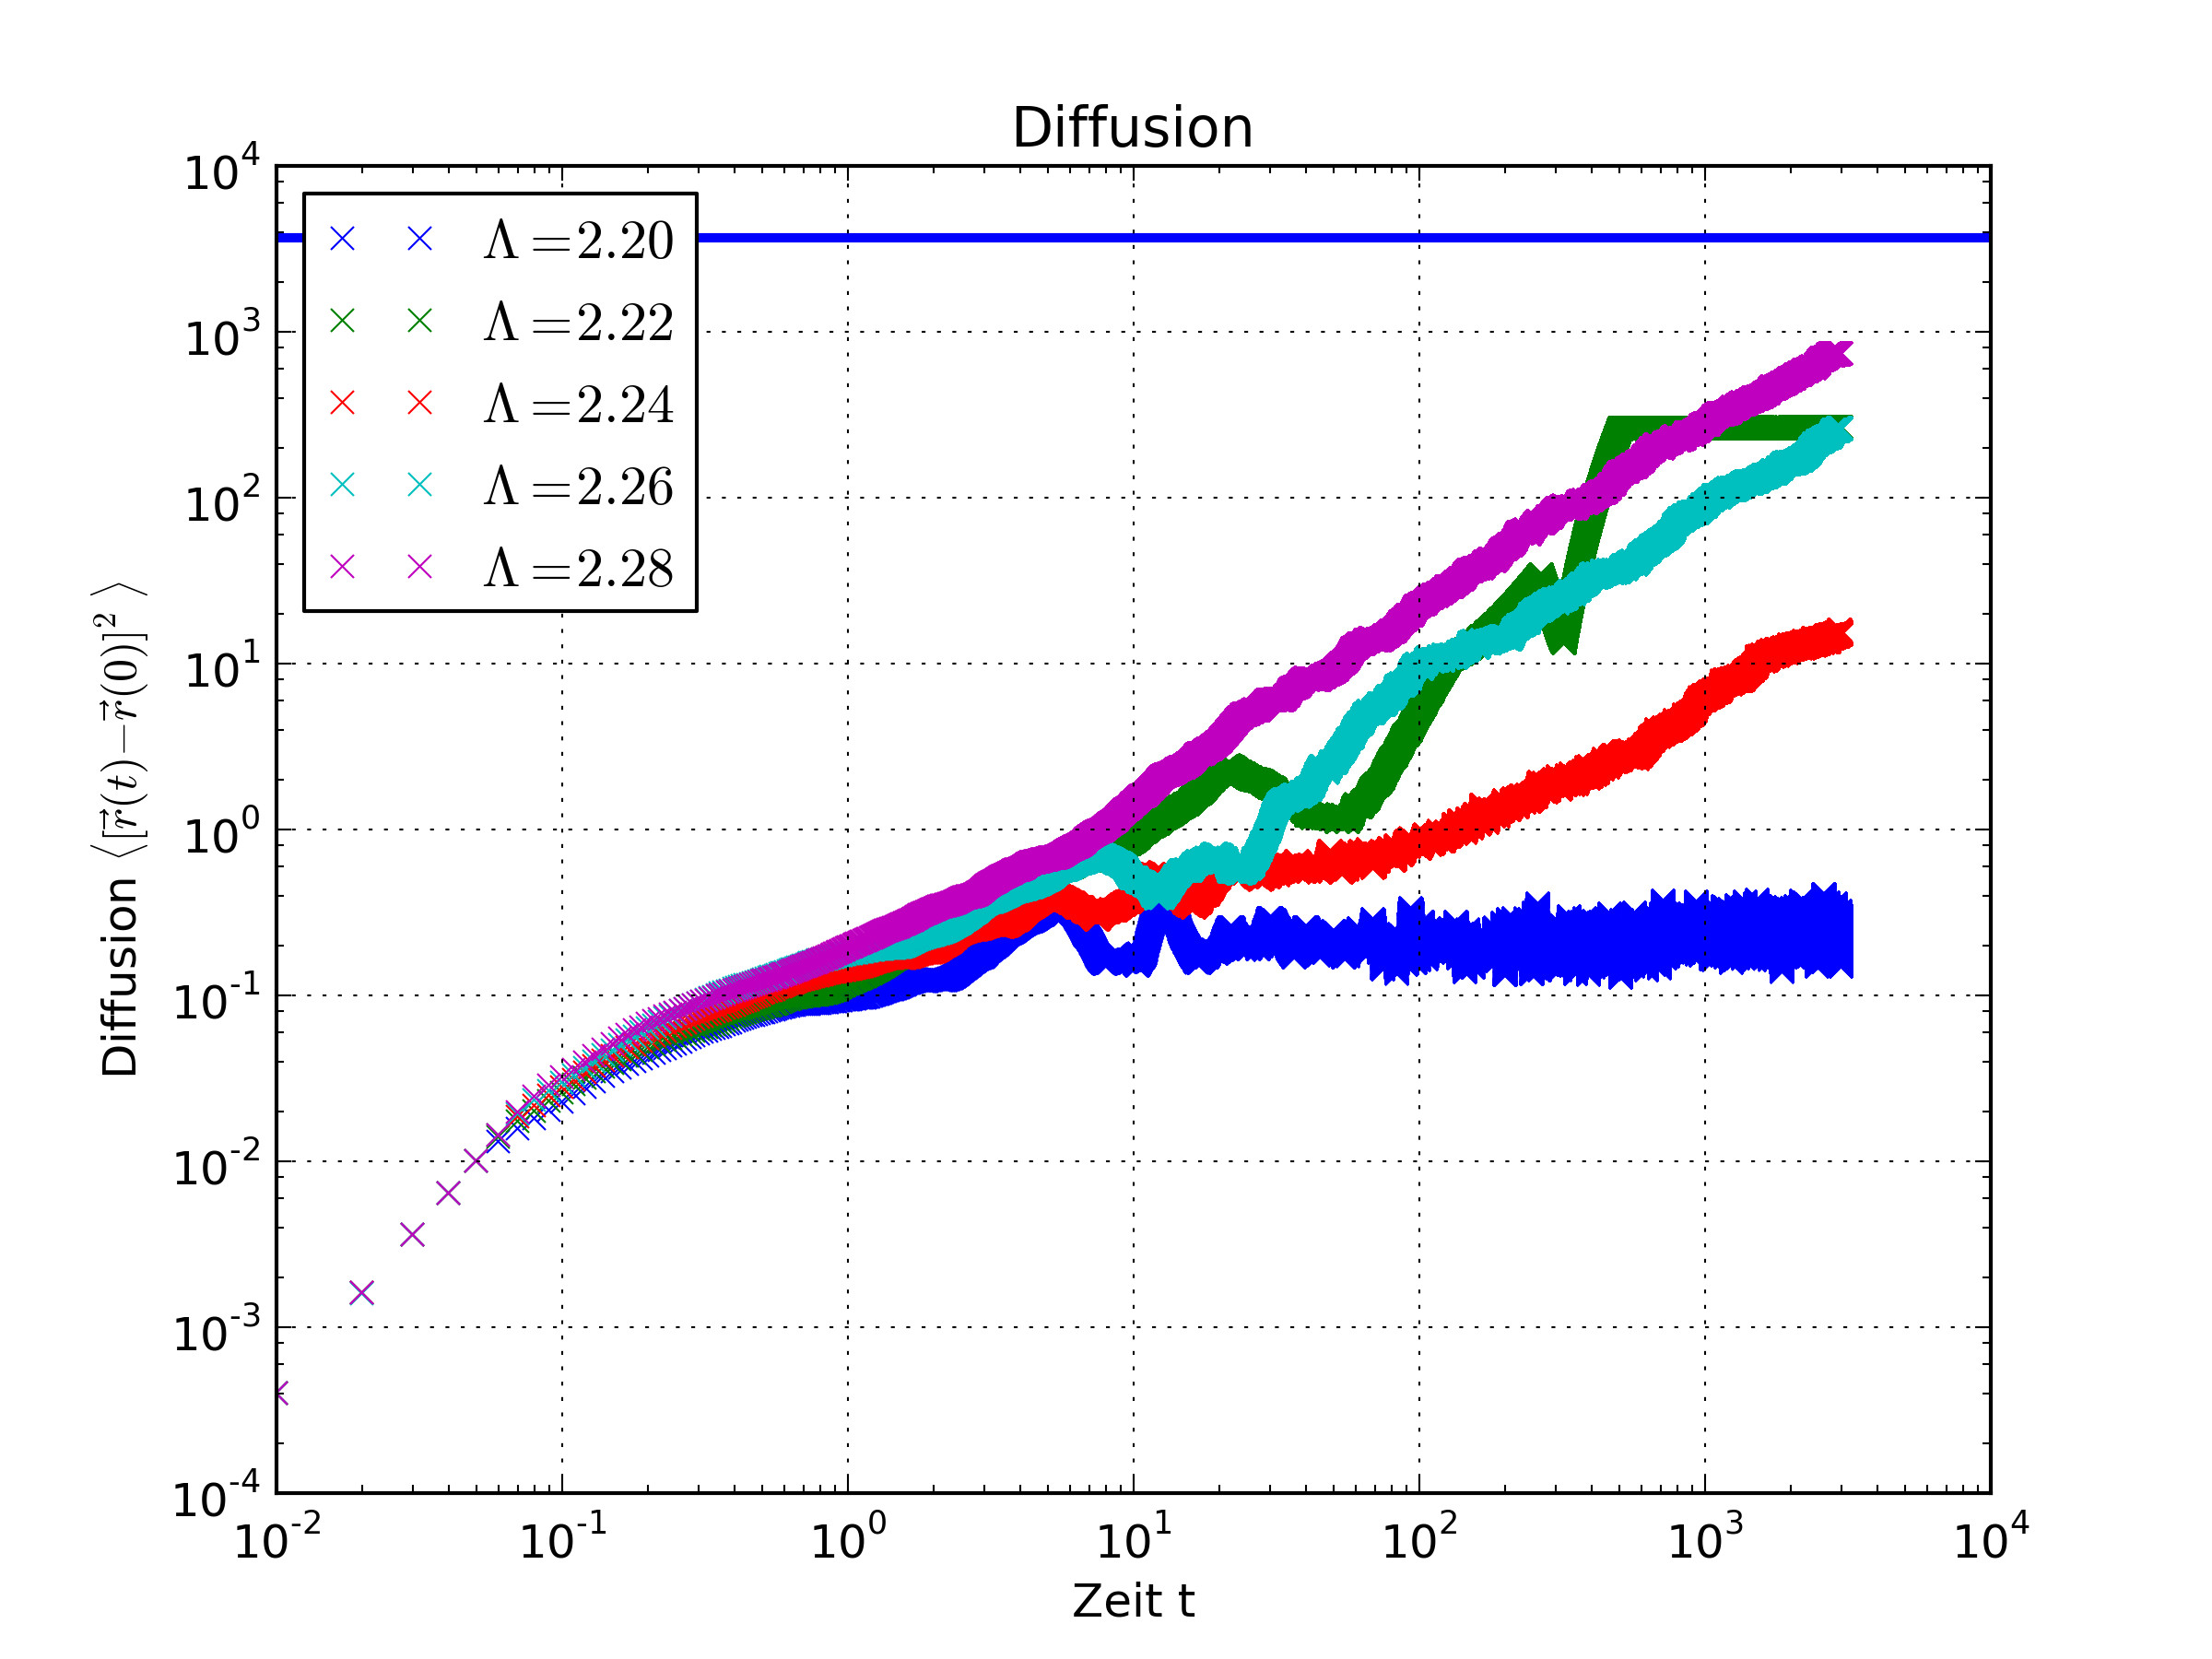
\includegraphics[width=0.70\textwidth]{img/A3_diffusion.png}
	\caption{Dargestellt ist das Diffusionsverhalten bei verschiedenen Gitterabst�nden. Bis zum ersten Sto� l�sst sich bei allen Dichten eine ballistische Diffusion feststellen. Ein Phasen�bergang, das hei�t eine �nderung des Diffusionsverhaltens von beschr�nkt auf diffusiv, l�sst sich zwischen $\Lambda=2.20-2.28$ beobachten. Die �berlagerung der festen und der fl�ssigen Phase w�hrend des Schmelzens f�hrt zu einer undefinierten Diffusionserscheinung.}
	\label{fig:A3_diffusion}
\end{figure}

Bis zum ersten Teilchensto� ist ein ballistisches Diffusionsverhalten zu beobachten. Danach sollte f�r den gasf�rmigen beziehungsweise fl�ssigen Zustand normales diffusives Verhalten beobachtbar sein. F�r den festen Zustand ergibt sich durch die Brown'sche Molekularbewegung ein beschr�nktes Verhalten. In \fref{fig:A3_diffusion} kann deswegen ein Phasen�bergang f�r $\Lambda=2.20-2.28$ vermutet werden. F�r $\Lambda=2.20$ entspricht die Steigung einem beschr�nkten Verhalten - f�r $\Lambda=2.28$ einem diffusiven. Dazwischen l�sst sich keine genaue Zuordnung treffen. Dies r�hrt daher, dass w�hrend des "`Schmelzens"' sowohl die feste als auch die fl�ssige Phase koexistieren. Diese �berlagerung der beiden Zust�nde f�hrt zu einer undefinierte Diffusionserscheinung.

\section{Paar-Korrelationsfunktion}
Zur �berpr�fung der Ergebnisse aus dem vorherigen Abschnitt wird auch noch die Paarkorrelationsfunktion der verschiedenen Konfigurationen untersucht. Die Paarkorrelationsfunktion in zwei Dimensionen ist wie folgt definiert: \cite{rapaport2004} und \cite{eibl2012}:
\begin{equation}
g(r_n) = \frac{h_n L_x L_y}{\pi N^2 r_n \Delta r}
\end{equation}
wobei $L_x$ und $L_y$ die Ausdehnung der Simulationsbox, $N$ die Gesamtzahl der Teilchen, $h_n$ die Anzahl der Teilchen im Abstand $r$ mit $(n-1)\Delta r<r<n\Delta r$, $r_n=(n+\frac{1}{2})\Delta r$ und $\Delta r$ die Diskretisierung des Abstands ist.

\begin{figure}[!ht]
	\centering
		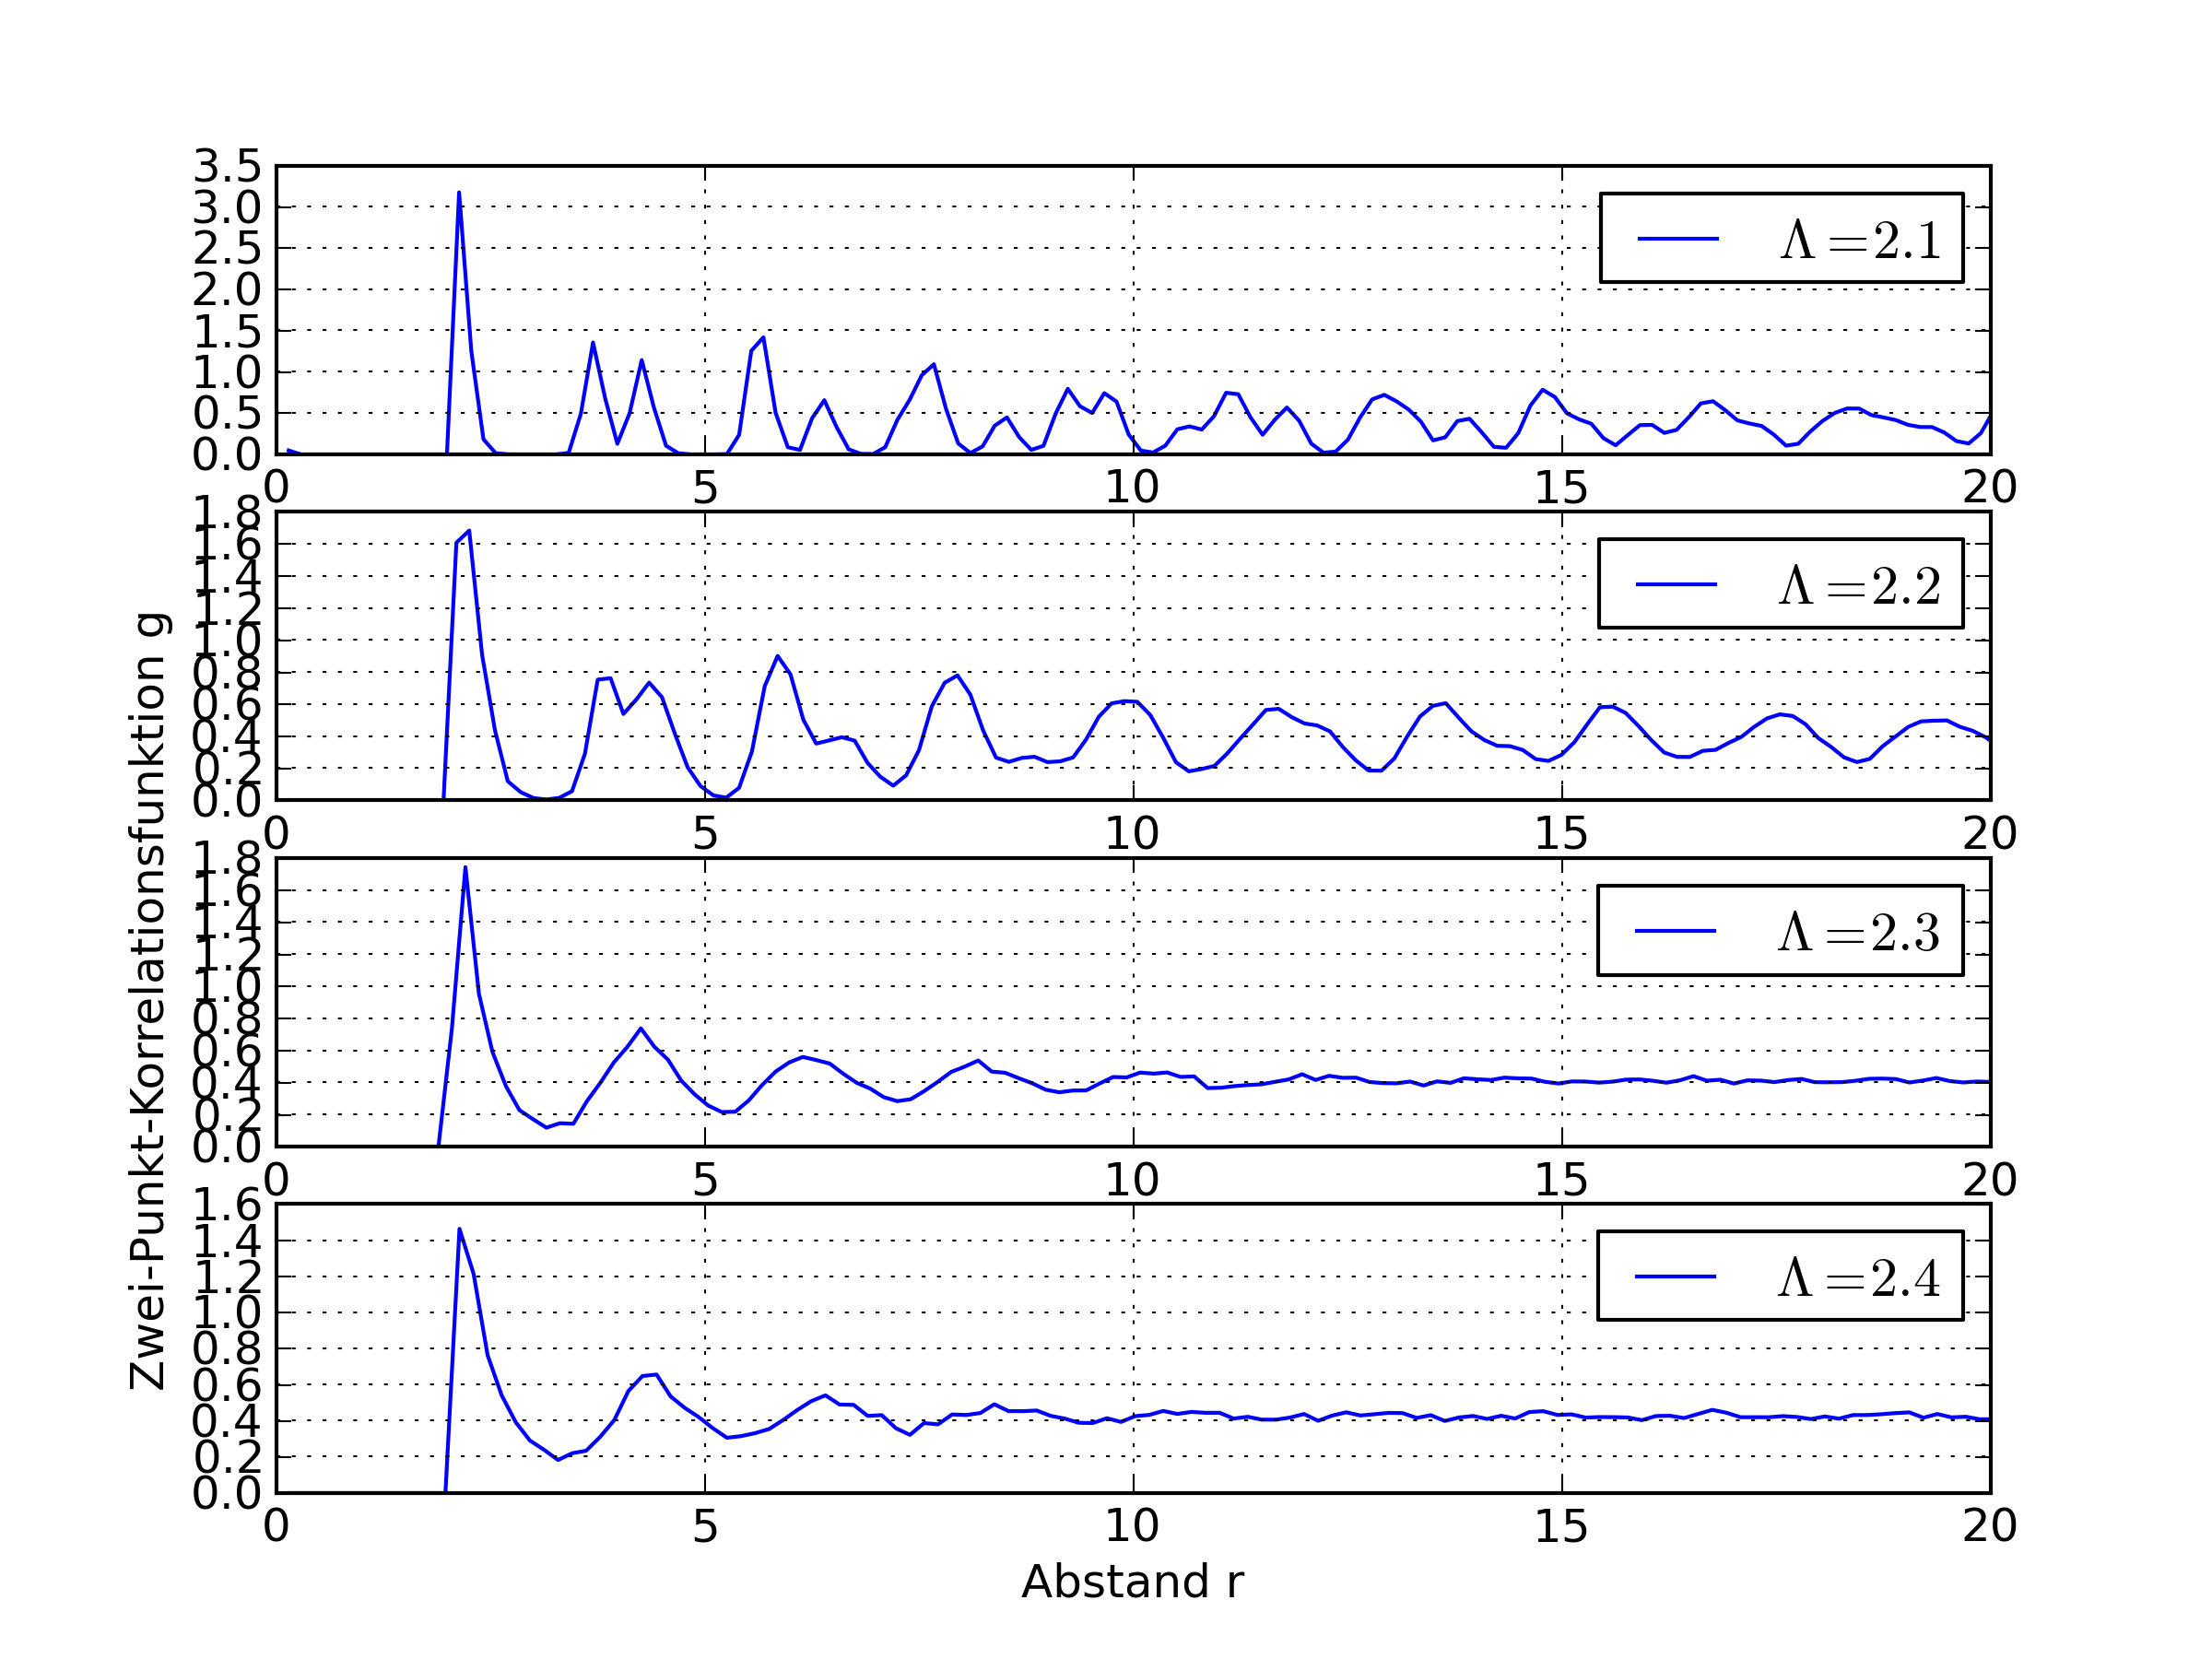
\includegraphics[width=0.70\textwidth]{img/A3_korrelation.png}
	\caption{Es l�sst sich beobachten, dass die strenge Ordnung des Kristallgitters f�r abnehmende Dichte - zunehmendem $\Lambda$} - verloren geht. Dies entspricht einem Phasen�bergang von fest nach fl�ssig.
	\label{fig:A3_korrelation}
\end{figure}

Die Ergebnisse der Paarkorrelation in \fref{fig:A3_korrelation} best�tigen die Vermutung, die durch Beobachtung des Diffusionsverhaltens aufgestellt worden ist.